\documentclass{article} % For LaTeX2e
\usepackage{nips15submit_e,times}
\usepackage{hyperref}
\usepackage{url}
\usepackage[cmex10]{amsmath}
\usepackage{array}
\usepackage{graphicx}
\usepackage{csquotes}
\usepackage{filecontents}
\usepackage{subcaption}

%\documentstyle[nips14submit_09,times,art10]{article} % For LaTeX 2.09


\title{Multi-Layer Neural Networks}


\author{
Christian Koguchi \\
PID: A10910223 \\
\And
Daniel Reznikov \\
PID: A12440386 \\
}



\newcommand{\fix}{\marginpar{FIX}}
\newcommand{\new}{\marginpar{NEW}}

\nipsfinalcopy % Uncomment for camera-ready version

\begin{filecontents}{biblio.bib}
@inproceedings{LeCun:1998:EB:645754.668382,
 author = {LeCun, Yann and Bottou, L{\'e}on and Orr, Genevieve B. and M\"{u}ller, Klaus-Robert},
 title = {Efficient BackProp},
 booktitle = {Neural Networks: Tricks of the Trade, This Book is an Outgrowth of a 1996 NIPS Workshop},
 year = {1998},
 isbn = {3-540-65311-2},
 pages = {9--50},
 numpages = {42},
 url = {http://dl.acm.org/citation.cfm?id=645754.668382},
 acmid = {668382},
 publisher = {Springer-Verlag},
 address = {London, UK, UK},
}
\end{filecontents}




\begin{document}

\maketitle


\begin{abstract}
In this report, we explore the ``tricks of the Neural Network trade" starting from our softmax regression solution to the previous homework.  We extend our network to support different activation functions, weight initializations, and network topologies.  We achieve nearly state-of-the art results with our best models hitting 99.7\% accuracy on the validation set and 97.4\% on the independently sourced test set.   
\end{abstract}



%%%%%%%%%%%%%%%%%%%%%%%%%%% Introduction 

\section*{Introduction}
The dataset that we are trying to classify is the classic MNIST dataset (sourced from Yann LeCun)\cite{Lecun}.  We aim to explore network topologies of various configurations for multi-layer perceptrons.  We implement efficient backpropogation of gradient descent manually.  We explore many common tricks of the trade and their sensitivity to hyperparameters and initial conditions.  In sum, this work crystallized our understanding of foundational neural network concepts.  What follows is an instructive discussion about our learning.  


%%%%%%%%%%%%%%%%%%%%%%%%%%% Methods  
\section*{Methodology}
\subsection*{Classification}

\begin{itemize}
\item \textbf{\textit{Lazy-Man Normalization:}} Pre-process the images by dividing by 127 and subtract 1, thereby moving all pixel values to the ranges [-1, 1]. 
\item \textbf{\textit{Hidden Layer}}: initialize the network with 1 hidden layer with 64 hidden units.  
\item \textbf{\textit{Numerical Gradient Checking}}: to validate our backpropogation algorithm implementation, we compare individual weight updates against the numerical approximation.
\item \textbf{\textit{Mini-Batch}}: we expose the hyperparameter \textit{batch-size} that allows us to separate the training set into small batches.  We update and calculate the gradient per batch.  We explore the impact of mini-batching by analyzing our accuracy scores on a withheld validation set of 10,000 randomly selected training images.  
\item \textbf{\textit{Grid Search}}: we implement brute-force grid search by manually searching over the space of learning rates and annealing parameters.  We do a search over the log-space characterized by the following intervals: $\{\eta \in [0.01, 0.00001], \ \ T \in [1, 1000] \}$. 
\end{itemize}  

\newpage

\subsection*{Tricks of the Trade}

\begin{itemize}
\item \textbf{\textit{Performance Metrics:}} We select a 97\% accuracy as a good threshold to benchmark our models.  We chose our two statistics because they independently measure interesting behavior.  Wall-Clock time is intrinsically valuable to the end-user because it represents the real cost to training.  Epochs to train give insight into how the experiment setup is able to lend itself to the model converging.
\item \textbf{\textit{Shuffling After Epochs}}: we randomly permute our training data before splitting into mini-batches.  
\item \textbf{\textit{Tanh Hidden Activation Function}}: to compare different members of the sigmoid class of functions, we implement the hyperbolic tangent function and use it for the activation for our hidden nodes.  These experiments were highly sensitive to initial weight conditions, so we invested great effort in tuning initial conditions.  The motivation for the tanh function is so that the hidden layer outputs have an average value of approximately 0 whereas the sigmoid will not.  
\item \textbf{\textit{Initial Weight Setup}}: we further our analysis by initializing our weights to a normal distribution with mean = 0 and standard deviation = $\frac{1}{\sqrt{\text{fan-in}}}$.  The fan-in is the number of connections from the previous layer.
\item \textbf{\textit{Momentum}}: leveraging the intuition from Lecun's `98 paper on momentum, we implement a momentum term that increases the step of the gradient with a term that is proportional to the running average of the gradients in the previous iterations.  
\end{itemize}

\subsection*{Experiments with Network Topology}

\begin{itemize}
\item \textbf{\textit{Hidden Unit Exploration}}: We halve the number of hidden units to 32 and double the hidden units to 128.  We profile our results by again measuring the wall-clock time and epochs to achieve a validation accuracy of 97\%.
\item \textbf{\textit{Hidden Layer Exploration}}: We add another hidden layer with the same number of hidden nodes (64) as the first layer.  Both layers have a bias term that is not connected to the previous layer.  
\end{itemize}

\subsection*{Additional Experiments}
\begin{itemize}
\item \textbf{\textit{ReLu Activation Function}}: We include the use of the ReLu activation function for our hidden units and again monitor the performance against our previous experiments in terms of wall-clock time and epochs.
\end{itemize}

\section*{Results}

\textbf{\textit{Numerical Gradient Checking}} \\ 

To validate backpropagation, we imploy a hook in our code that computes the numerical gradient as follows: $$\frac{\partial E^n}{\partial w_{ij}} \approx \frac{E^n(w_{ij} + \epsilon) - E^n(w_{ij} - \epsilon)}{2\epsilon}$$ \\ 

We test with $\epsilon = 0.01$.  We found that the difference between the numerically computed gradients and the backprop gradients are between $[10^{-5}, \ 10^{-7}]$ for various model parameters and we found that the difference is always $O(\epsilon^2)$, as expected. \\


{\renewcommand{\arraystretch}{1.5}
\begin{table}[h!]
\centering
\caption{Numerical Gradient Checking}
\label{my-label}
\begin{tabular}{|l|l|l|l|l|} \hline
$\epsilon = 10^{-2}$ & Numerical Gradient & Backprop Gradient & Difference                           & $O(\epsilon^2)$  \\ \hline
Input Bias(0, 63)                    & -0.027          & -0.028         & -1.855$\times10^{-7}$ & T                             \\ \hline
Input Bias(0, 4)                     & 0.311           & 0.311          & -6.823$\times10^{-6}$     & T                             \\ \hline
Output Bias(0, 3)                    & -10.082         & -10.083       & 8.523$\times10^{-5}$   & T                             \\ \hline
Output Bias(0, 4)                    & -1.310           & -1.311          & 9.444$\times10^{-5}$     & T                             \\ \hline
$w_{hidden}$(3, 4)                  & 0.322           & 0.322          & 3.685$\times10^{-7}$     & T                             \\ \hline
$w_{hidden}$(64, 63)                & -0.310          & -0.309         & 5.960$\times10^{-7}$    & T                             \\ \hline
$w_{output}$(2, 2)                  & -0.364          & -0.364         & 4.226$\times10^{-6}$    & T                             \\ \hline
$w_{output}$(37, 7)                 & 1.138           & 1.382           & 5.120$\times10^{-5}$    & T                             
\\ \hline
\end{tabular}
\end{table}

\newpage

\textbf{\textit{Experiment Results}} \\ 


We found that all configurations of our experiments can be tuned to achieve very high accuracies.  Our results follow:

{\renewcommand{\arraystretch}{1.5}
\begin{table}[h!]
\centering
\caption{Results to get 97\% Validation Accuracy}
\label{my-label}
\begin{tabular}{|p{2cm}|p{6cm}|p{2cm}|p{1.5cm}|}
\hline
\textbf{Experiment No.}            & \textbf{Description}                                                          & \textbf{Wall-Clock Time [secs]} & \textbf{Epochs} \\ \hline
1 & Mini-Batch of 128 + Weights from a Uniform Distribution{[}-1, 1{]} & 24.2123                                              & 12                                  \\ \hline
2 & Shuffling after Epochs and Averaging the Gradient                                         & 16.8966                                              & 8                                  \\ \hline
3 & Using Tanh Activation Function                                                            & 38.6009 	 & 18                                  \\ \hline
4 & Initialize Weights $w \sim \mathcal{N} \bigg(0, \  \frac{1}{\sqrt{fan-in}} \bigg)     $ & 17.9693                                              & 8                                   \\ \hline
5 & Momentum $\alpha$ = 0.9                                                                     & 17.5322 & 7                                   \\ \hline
6 & Halving Hidden Units to 32                                                                &  22.2573 & 14                                  \\ \hline
7 & Doubling Hidden Units to 128                                                              & 33.542 & 8                                   \\ \hline
8 & Using 2 Hidden Layers                                                                     & 9.0301                                               & 24                                    \\ \hline
9 & Using ReLu Activation Function                                                       & 13.2923 & 7                                    \\ \hline
\end{tabular}
\end{table}

\begin{figure*}[h!]
\captionsetup[subfigure]{labelformat=empty}
    \centering
    \begin{subfigure}[t]{0.5\textwidth}
        \centering
        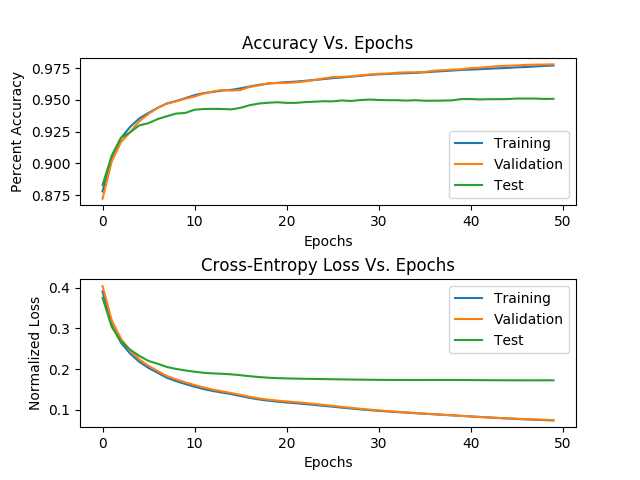
\includegraphics[scale=0.48]{3e.png}
        \caption{Experiment 1: Mini-batching 128}
    \end{subfigure}%
    ~ 
    \begin{subfigure}[t]{0.5\textwidth}
        \centering
        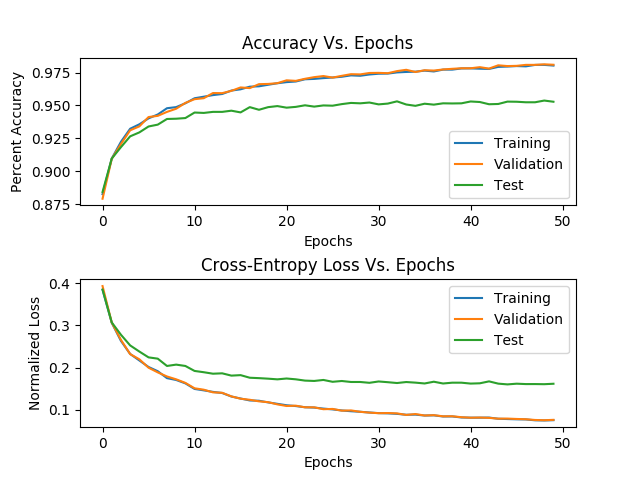
\includegraphics[scale=0.48]{4a.png}
        \caption{Experiment 2: Shuffling after Epochs/Averaging}
    \end{subfigure}
\end{figure*}


\begin{figure*}[h!]
\captionsetup[subfigure]{labelformat=empty}
    \centering
    \begin{subfigure}[t]{0.5\textwidth}
        \centering
        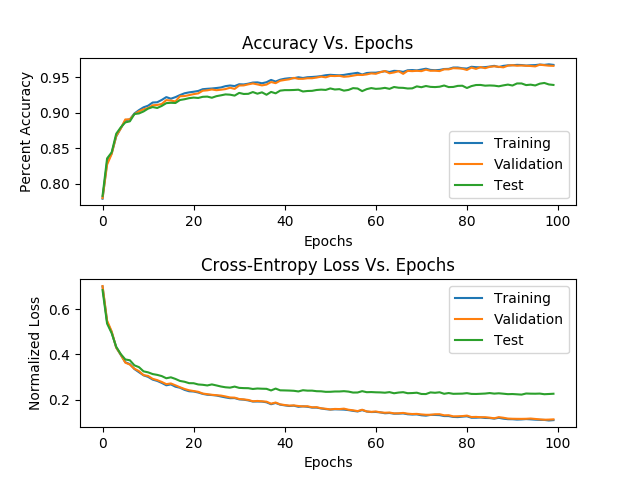
\includegraphics[scale=0.48]{4B.png}
        \caption{Experiment 3: Tanh Activation Function}
    \end{subfigure}%
    ~ 
    \begin{subfigure}[t]{0.5\textwidth}
        \centering
        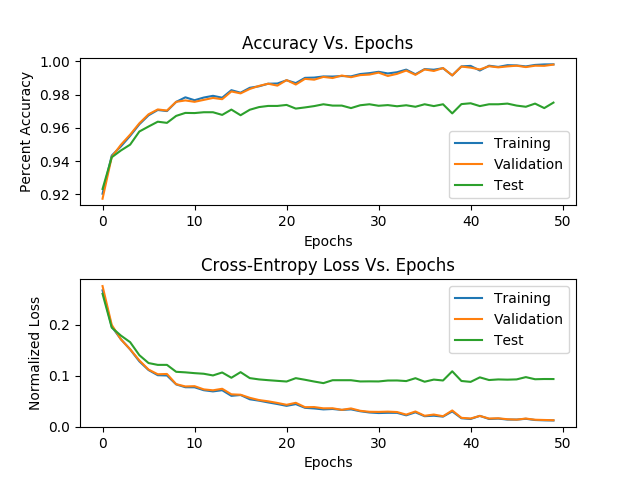
\includegraphics[scale=0.48]{4C.png}
        \caption{Experiment 4: Initializing Weights using Fan-In}
    \end{subfigure}
\end{figure*}

\begin{figure*}[h!]
\captionsetup[subfigure]{labelformat=empty}
    \centering
    \begin{subfigure}[t]{0.5\textwidth}
        \centering
        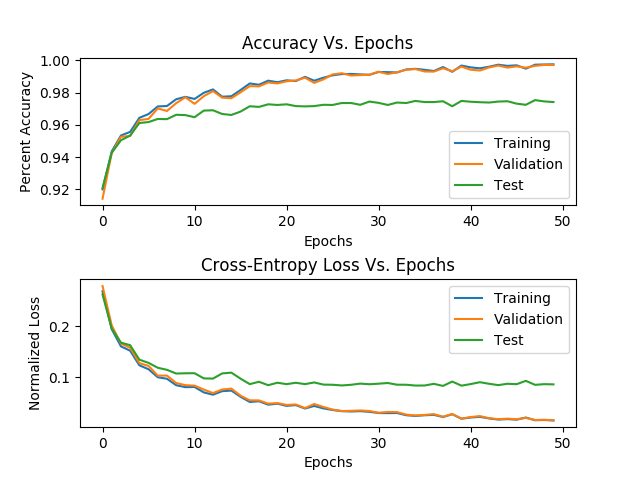
\includegraphics[scale=0.48]{4D.png}
        \caption{Experiment 5: Momentum}
    \end{subfigure}%
    ~ 
    \begin{subfigure}[t]{0.5\textwidth}
        \centering
        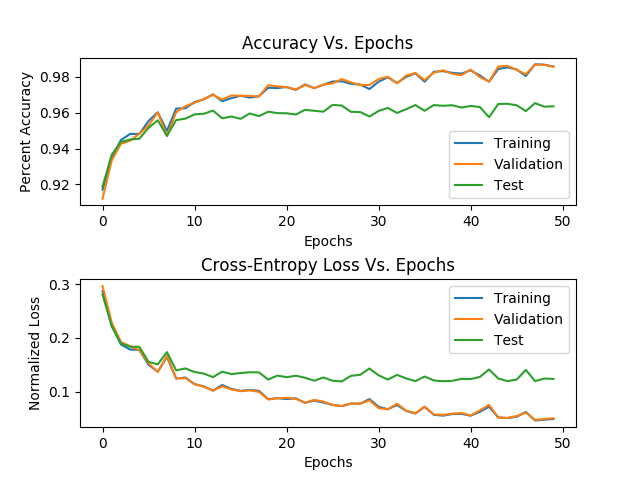
\includegraphics[scale=0.48]{5A_1.png}
        \caption{Experiment 6: Halving Hidden Units}
    \end{subfigure}
\end{figure*}

\begin{figure*}[h!]
\captionsetup[subfigure]{labelformat=empty}
    \centering
    \begin{subfigure}[t]{0.5\textwidth}
        \centering
        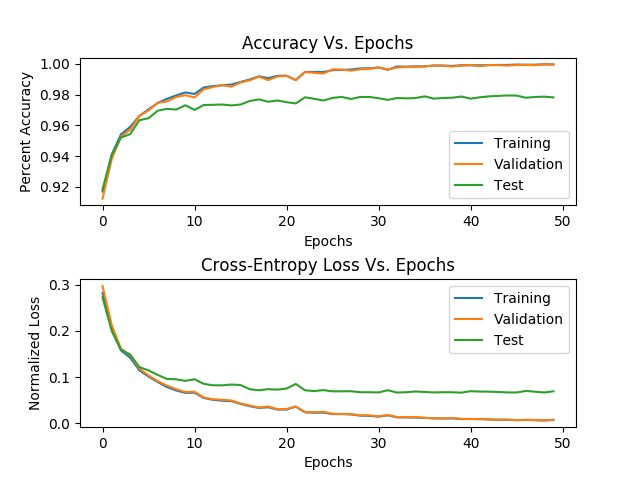
\includegraphics[scale=0.48]{5A_2.png}
        \caption{Experiment 7: Doubling Hidden Units}
    \end{subfigure}%
    ~ 
    \begin{subfigure}[t]{0.5\textwidth}
        \centering
        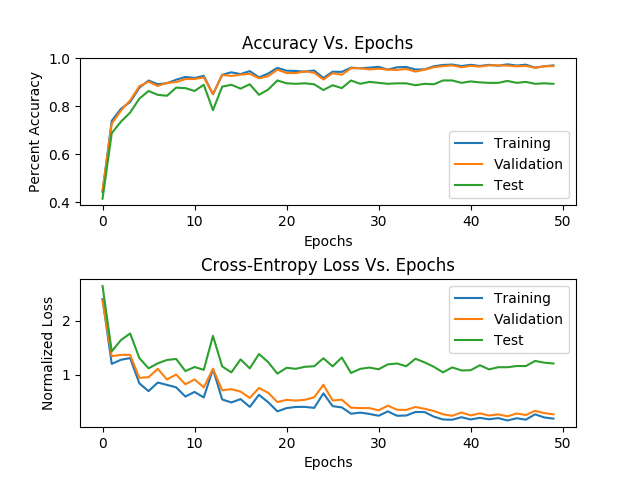
\includegraphics[scale=0.48]{5B.png}
        \caption{Experiment 8: Two Layer Network}
    \end{subfigure}
\end{figure*}




\newpage


\section*{Discussion}

\begin{itemize}
\item \textbf{\textit{Mini-Batch}}: We are pleasantly surprised by how mini-batching greatly accelerates the rate of learning.  By exploiting the stochastic numerical processes, we are able to converge rapidly upon an optimal solution due to the redundancy in the training set.  This made training our large dataset more manageable. While we didn't experiment much with the batch size, we found that the initial setup of 128 was already a good balance between performance and being large enough to provide a meaningful sample of our training data. 
\item \textbf{\textit{Shuffling}}: To further exploit the randomness in our stochastic approach, we introduce shuffling after each epoch.  This means our learning is more robust because the class distribution is rigorously randomized within mini-batches.  Our results show that while the wall-clock time was stable, the number of epochs decreased by 50\%. 
\item \textbf{\textit{Tanh}}: Yann LeCun's paper developed our intuition as to why the tanh function will be more efficient during learning.  In comparison to the logistic sigmoid, the output weights of the tanh activation function will on average gravitate towards 0 whereas the range of the logistic sigmoid is always positive.  During backpropagation, this means that the weight change rules can move in both positive and negative directions.  We found that the tanh function was markedly better, achieving the 97\% accuracy in 6 epochs as compared to 22 and in 10.60 seconds. 
\item \textbf{\textit{Momentum}}: The loss function is locally convex, so the intution behind the momentum term is that it will push our model over local minima allowing it to converge faster and with higher accuracy.  Despite this intuition, we did not find significant improvements in either of our performance metrics (see table above).  We suspect this is happening because our other hyperparameters are already compensating sufficiently for fast convergence.  
\item \textbf{\textit{Halving Hidden Units}}: Halving the number of hidden units does not decrease the model accuracy but increases the wall-clock time by about 50\% and the number of epochs by about 100\%.  From this we conclude that it was not by happenstance that we were asked to use 128 hidden units because that seems to be the sweet spot.  
\item \textbf{\textit{Doubling Hidden Units}}: Doubling the number of units in the hidden layer to 128 resulted in the same training epochs (8) but more wall-clock time (50\% increase).  Doubling the number of hidden units doubles the number of weights.  The number of training epochs doesn't change because multiple neurons may be learning the same features.  
\item \textbf{\textit{Using 2 Hidden Layers}}: Our intuition told us that two hidden layers should train longer but produce better models.  Our hypothesis was confirmed by obversving that we can achieve near state-of-the-art performance while epochs remained the same and training time in seconds doubles.
\item \textbf{\textit{ReLu}}: We were pleasantly surprised that the ReLu activation function converged much more quickly than previous experiments and converged for most choices of hyperparameters. It performs approximately 30\% faster on wall-clock time and the same number of epochs as using the tanh activation.  
\end{itemize}

\section*{Conclusion}

First, we are very grateful for this assignment because we have learned many interesting intuitions about neural networks.  The most profound learnings were the influence of the tanh activation function and the sensitivity of these networks to weight initializations.  We appreciated deeply that each subsequent experiment clearly demonstrated improvements over each predecessor.  Lecun's whitepaper and our lectures greatly enhanced our intuition about network topologies and tricks of the trade.  The rigorous mathematical analysis requried to both apply the recursive backpropagation was a rewarding challenge.  In sum, we are very pleased to report models that achieve 97.4\% validation set accuracy.  


\section*{Individual Contributions}

Christian did much of the heavy lifting for the derivation for backprop.  Christian was instrumental in vectorizing our code and to prototyping backpropagation.  Christian helped with the write-up.  Christian implemented grid-search to find the optimal parameters for our models.  

Daniel architected our code to be modular, reusable, and professional.  He enforced the Extreme-Programming paradigm and code style.  Daniel spent much effort on debugging and training our models.  Daniel worked extensively on the write-up.  



\newpage

\section*{Appendix}

For reproducibility, we provide our model hyperparameters as follows.


\begin{table}[h!]
\small
\centering
\caption{Model Hyperparameter Values}
\label{my-label}
\begin{tabular}{|p{1.5cm}|p{1.3cm}|p{1.3cm}|p{1cm}|p{1cm}|p{1.7cm}|p{1.5cm}|p{1cm}|p{1cm}|}
\hline
\textbf{Experiment No.} & \textbf{Annealing} & \textbf{Learning Rate} & \textbf{Shuffle} & \textbf{Hidden Activation} & \textbf{Weight Init.}    & \textbf{Momentum} & \textbf{Hidden Nodes} & \textbf{Hidden Layers} \\ \hline
1                       & 100                & 0.01                   & False            & Logistic                   & uniform {[}-0.5, 0.5{]}  & False             & 64                    & 1                      \\ \hline
2                       & 10                 & 0.01                   & True             & Logistic                   & uniform {[}-0.5, 0.5{]}  & False             & 64                    & 1                      \\ \hline
3                       & 1                  & 0.001                  & True             & Tanh                       & uniform {[}-0.5, 0.5{]}  & False             & 64                    & 1                      \\ \hline
4                       & 600                & 0.001                  & True             & Tanh                       & $\mathcal{N} \big(0, \frac{1}{\sqrt{\text{fan-in}}} \big)$  & False             & 64                    & 1                      \\ \hline
5                       & 10                 & 0.0005                 & True             & Tanh                       & $\mathcal{N} \big(0, \frac{1}{\sqrt{\text{fan-in}}} \big)$ & True              & 64                    & 1                      \\ \hline
6                       & 100                & 0.00005                & True             & Tanh                       & $\mathcal{N} \big(0, \frac{1}{\sqrt{\text{fan-in}}} \big)$ & True              & 32                    & 1                      \\ \hline
7                       & 750                & 0.00005                & True             & Tanh                       & $\mathcal{N} \big(0, \frac{1}{\sqrt{\text{fan-in}}} \big)$ & True              & 128                   & 1                      \\ \hline
8                       & 100                  & 0.00001                      & True             & Tanh                       & $\mathcal{N} \big(0, \frac{1}{\sqrt{\text{fan-in}}} \big)$ & True              & 64                    & 2                      \\ \hline
9                       & 200                  & 0.0003                      & True             & ReLu                       & $\mathcal{N} \big(0, \frac{1}{\sqrt{\text{fan-in}}} \big)$ & True              & 64                    & 1                      \\ \hline
\end{tabular}
\end{table}


































\end{document}